\documentclass[runningheads,a4paper]{llncs}

\usepackage{url}


%Preamble File for Random Regression Paper

%\usepackage{times}

%Theorems and such

%\usepackage{amsthm}

%\newtheorem{theorem}{Theorem}
%\newtheorem{observation}{Observation}
%\newtheorem{proposition}{Proposition}
%\newtheorem{definition}{Definition}

%\newtheorem{theorem}{Theorem}[section]
%\newtheorem{observation}{Observation}[section]
%\newtheorem{proposition}{Proposition}[section]
%\newtheorem{definition}{Definition}[section]

\usepackage[ruled,vlined]{algorithm2e}
\usepackage{algorithmic}
%\usepackage{amsthm}
\usepackage{amsmath}
\usepackage{amsfonts}
\usepackage{amssymb}
\usepackage{graphicx}
\usepackage{url}
\usepackage{subfigure}
\usepackage{epstopdf}
%\setcounter{MaxMatrixCols}{30}
%\usepackage[ruled,vlined]{algorithm2e}
%\usepackage{algorithmic}
\usepackage{multirow}
\usepackage{subfigure}
\usepackage{ifthen}
\DeclareMathOperator*{\argmax}{argmax}
\DeclareMathOperator*{\argmin}{argmin}
%\DeclareMathOperator{\pattern}{\pi}
\DeclareMathOperator{\Poly}{\mathbf{\mathrm{P}}}
\DeclareMathOperator{\RP}{\mathbf{\mathrm{RP}}}
%\DeclareMathOperator{\FP}{\mathbf{\mathrm{FP}}}
\DeclareMathOperator{\NP}{\mathbf{\mathrm{NP}}}
%\DeclareMathOperator{\E}{\mathbb{E}}

\newcommand{\defterm}{\textbf}

\renewcommand{\d}{\mathbf{d}}

\newcommand{\ZZ}{\mathbf{Z}}

\newcommand{\indep}{\ensuremath{\perp{}\!\!\!\!\!\!\!\perp{}}}
\newcommand{\dep}{\ensuremath{{\perp{}\!\!\!\!\!\!\!\not  \perp{}}}}
%\renewcommand{\L}{\mathcal{L}}

% variables denoting sets of nodes
\newcommand{\BN}{B} % Bayes net
\newcommand{\V}{V} 
\newcommand{\partC}{\mathcal{C}}
\newcommand{\pattern}{\pi}
% for population variables
\newcommand{\A}{\mathbb{A}}
\newcommand{\B}{\mathbb{B}}
\newcommand{\C}{\mathbb{C}}
\newcommand{\U}{\mathbb{U}}
%maybe use P, R as well??
\renewcommand{\P}{P}
\newcommand{\R}{R}
% values of Pop variables = constants
\renewcommand{\a}{a}
\renewcommand{\b}{b}
\renewcommand{\c}{c}

%%%
% for terms = nodes in Functor Bayes Net.
\newcommand{\X}{X}
\newcommand{\Y}{Y}
\newcommand{\Z}{Z}
% Next three are currently only ones eligible for \Mrange and \Prange
\newcommand{\TT}{T}
\newcommand{\TI}{\mathsf{T}}
\newcommand{\UT}{U}
\newcommand{\UI}{\mathsf{U}}
\newcommand{\VT}{V}
\newcommand{\VI}{\mathsf{V}}
\newcommand{\W}{W}
%syntax for values
\newcommand{\z}{z}
\renewcommand{\v}{v}
\newcommand{\x}{x}
\newcommand{\y}{y}
\newcommand{\p}{p}
\newcommand{\s}{s}
% Values tied to terms
\newcommand{\TV}{t}
\newcommand{\TTuple}[1][0.0ex]{\vec{t}\hspace{#1}}
\newcommand{\UV}{u}
\newcommand{\UTuple}[1][0.0ex]{\vec{u}\hspace{#1}}
\newcommand{\VV}{v}
\newcommand{\VTuple}{\vec{v}}
%%%
\newcommand{\weight}{w} % weights
% Formulas
\newcommand{\TF}{\vec{T}}
\newcommand{\UF}{\vec{U}}
\newcommand{\VF}{\vec{V}}
%\newcommand{\TF}{\phi}
%\newcommand{\UF}{\psi}
%\newcommand{\VF}{\omega}
% Database (which is always fully-grounded)
\newcommand{\DB}{\FG{\Delta}}
\newcommand{\QC}{\FG{\Lambda}}
\newcommand{\QCtarget}{\FG{\Lambda_{-\TI}}}
% to define a query conjunction of literals
\newcommand{\Qconj}{\Appendterm{\FG{\TT_{\grounding}} = \TV} {\QC}}

% Annotations marking degree of grounding
\newcommand{\UG}[2][0.0ex]{#2^{-}\hspace{#1}}
\newcommand{\PG}[2][0.0ex]{#2^{\prime}\hspace{#1}}
\newcommand{\FG}[2][0.0ex]{#2^{*}\hspace{#1}}

% Functions returning related terms
\newcommand{\MB}[1]{\mathrm{MB}(#1)}
\newcommand{\Pa}[1]{\mathrm{Pa}(#1)}
\newcommand{\Ch}[1]{\mathrm{Ch}(#1)}

% Grounding
\newcommand{\Ground}[1]{#1_\gamma}
\newcommand{\gndlink}{\backslash}

% Values in ranges of example functors
\newcommand{\Man}{\mathrm{M}}
\newcommand{\Woman}{\mathrm{W}}

% Adding a term to a formula
\newcommand{\sepcup}[1][0.5ex]{\hspace{#1}\cup\hspace{#1}}
\newcommand{\Setaddterm}[2]{#1 \sepcup #2}
\newcommand{\Appendterm}[2]{#1, #2}

% Values in the range of related terms
\newcommand{\Mrange}[1]{\ifthenelse{\equal{#1}{T}}{\TTuple_m}{\ifthenelse{\equal{#1}{U}}{\UTuple_m}{\ifthenelse{\equal{#1}{V}}{\VTuple_m}{\mbox{UNKNOWN
TERM ID}}}}}
\newcommand{\Prange}[1]{\ifthenelse{\equal{#1}{T}}{\vec{t}_{pa}}{\ifthenelse{\equal{#1}{U}}{\vec{u}_{pa}}{\ifthenelse{\equal{#1}{V}}{\vec{v}_{pa}}{\mbox{UNKNOWN
TERM ID}}}}}

\newcommand{\GroundPrange}[1]{\ifthenelse{\equal{#1}{T}}{\vec{t}_{pa,\grounding'}}{\ifthenelse{\equal{#1}{U}}{\vec{u}_{pa,\grounding'}}{\ifthenelse{\equal{#1}{V}}{\vec{v}_{pa,\grounding'}}{\mbox{UNKNOWN
TERM ID}}}}}


% Key functions
\newcommand{\joint}{p}
\newcommand{\jprob}[1]{\theta(#1)}
\newcommand{\cprob}[2]{\theta(#1|#2)}
\newcommand{\estcprob}[3]{\widehat{\theta}(#1|#2;#3)}
%\newcommand{\Gpvar}{\tilde{P}}
\newcommand{\Gpvar}{P}
\newcommand{\Gprob}[2]{\Gpvar(#1 | #2)}
\newcommand{\QFC}{QFC} % query family configuration
\newcommand{\Cvar}{\mathrm{n}}
\newcommand{\Fvar}{\mathrm{p}}
\newcommand{\Count}[2]{\Cvar\left[#1;#2\right]}
\newcommand{\CountC}[3]{\Cvar_{#3}\left[#1;#2\right]}
\newcommand{\Freq}[2]{\Fvar\left[#1;#2\right]}
\newcommand{\Relevant}[1]{#1^{\mathrm{r}}}
\newcommand{\Relcount}[2]{\Relevant{\Cvar}\left[#1;#2\right]}
\newcommand{\RelcountC}[3]{\Relevant{\Cvar_{#3}}\left[#1;#2\right]}
\newcommand{\Relfreq}[2]{\Relevant{\Fvar}\left[#1;#2\right]}
\newcommand{\RelfreqC}[3]{\Relevant{\Fvar_{#3}}\left[#1;#2\right]}
\newcommand{\Range}[1]{\mathrm{Ra}(#1)}
\newcommand{\Vars}[1]{\mathrm{Va}(#1)}
% no longer needed
%\newcommand{\Crossprod}[1]{\mathcal{X}}

%variables for sets of values
\newcommand{\setx}{\set{x}}
\newcommand{\sety}{\set{y}}
\newcommand{\setz}{\set{z}}


%statistics
\newcommand{\score}{S}
\newcommand{\parameters}{\mathit{par}}
\newcommand{\bic}{\mathit{BIC}}
%random variables and graphical models
% number of values in the domain of a random variable
% variables for BNs
\newcommand{\domvals}{k}
\newcommand{\nodevalue}{\x}
\newcommand{\parvalue}{\mathbf{\pi}} % a single assignment of values to a set of 
%parents
\newcommand{\parvals}{l} % number of values of parent state.
\renewcommand{\r}{r} % CP-table row
\newcommand{\nbhd}{{\mathsf {nbdh}}}
\newcommand{\child}{\mathit{child}}
\newcommand{\parent}{\mathit{pa}}
\newcommand{\parents}{\mathbf{pa}}
\newcommand{\Parents}{\mathbf{PA}}
\newcommand{\family}{F} % families, family formulas
\newcommand{\Target}{Y_{\target}}
\newcommand{\MBtarget}{\set{X}_{\target}} % Markov blanket of a target node.
\newcommand{\mbtarget}{\set{x}} % values for the markov blanket of a variable, vector-valued
\newcommand{\mbstates}{m} % number of states in Markov blanket
\newcommand{\vpi}{\mathbf{pa}} % for vectors of variable assignments
\renewcommand{\l}{\ell} % class label
\newcommand{\states}{r} % number of states of a variable
\newcommand{\ssize}{N} % number of rows in join table; size of sample
\newcommand{\frequency}{fr}
\newcommand{\pseudo}{\ast}
\newcommand{\counts}{+}
\newcommand{\weighted}{\ast}
\newcommand{\halpern}{H}
\newcommand{\instance}{I}

%logic notation
\newcommand{\functor}{f}
\newcommand{\fvalue}{v}
\newcommand{\variable}{X} % first-order variable
\newcommand{\population}{\mathcal{P}}
\newcommand{\entity}{x}
\newcommand{\formula}{\phi}
\newcommand{\formulas}{\mathcal{\phi}}
\newcommand{\conjunction}{\set{C}} % 
\newcommand{\outdomain}{V}
\newcommand{\literal}{\ell}
%conjunction of literals
\newcommand{\fterm}{\f} % open function term
\newcommand{\fterms}{F} % set of function terms, also nodes in JBN
\newcommand{\term}{\tau}
\newcommand{\terms}{\bs{\tau}}
\newcommand{\constant}{a}
\newcommand{\constants}{\bs{\constant}}
\newcommand{\gterm}{g} % ground term
\newcommand{\gterms}{\bs{\gterm}} %list of ground terms
\newcommand{\vterm}{x} % variable term
\newcommand{\vterms}{\bs{\vterm}} % list of variable terms
\newcommand{\assign}{A} % assignment of values to Bayes net
\newcommand{\grounds}{\#}
\newcommand{\grounding}{\gamma}
\newcommand{\groundall}{\Gamma}
\newcommand{\vars}{\mathit{Var}} % variables in a conjunction
\newcommand{\igraph}{I} % instance-level dependency graph.
\newcommand{\assignment}{\set{a}}
\newcommand{\atom}{\functor}
\newcommand{\gnode}{\alpha}
\newcommand{\gfamily}{\ground{f}}
\newcommand{\numformulas}{m}
% logic programs
\newcommand{\program}{\mathcal{B}}
\newcommand{\clause}{\mathcal{c}}
\newcommand{\head}{\mathit{head}}
\newcommand{\body}{\mathit{body}}
\newcommand{\crule}{\mathit{cr}} % combining rule
\newcommand{\level}{\mathit{level}} % rank of function symbols in LP

%datbase schema
\newcommand{\rcolumns}{R}
\newcommand{\ecolumns}{E}
\newcommand{\dtable}{T} % can't use \table. Generic database table
\newcommand{\datatable}{D} % generic data table, not necessarily part of database.
\newcommand{\jtable}{J} % join table
\newcommand{\Ejoin}{$J^{+}$}
\newcommand{\jtables}{m}
\newcommand{\rtable}{R} % relationship table
\newcommand{\etable}{E} % entity table.
\newcommand{\ttable}{X} % target table
\newcommand{\nextended}{n}
\newcommand{\row}{r}
\newcommand{\rows}{\mathit{rows}}
\newcommand{\col}{j}
\newcommand{\cols}{\mathit{cols}}
\newcommand{\unary}{\f} % to denote a unary or attribute function
\newcommand{\numatts}{u} % to denote the number of unary or attribute functions.
\newcommand{\g}{g} % alternative for function
\newcommand{\relational}{\mathbf{r}} % denotes a generic relational functors, can be both relationship or descriptive attribute of relationship
\newcommand{\Relation}{R} % denotes a generic boolean relation
% a special type of literal conjunction that assigns a value %to each variable
\newcommand{\class}{c} % the class attribute
\newcommand{\classifier}{\mathcal{C}}
\newcommand{\target}{t} % target object
\newcommand{\feature}{f} % feature or desc attribute of object or link
\newcommand{\features}{\bs{f}} % features 
\newcommand{\attribute}{a} % nonclass attribute of target object
\newcommand{\attributes}{\bs{a}}
\newcommand{\rels}{\bs{R}} % chain of relationships.
\newcommand{\maxpath}{\rho}

%special functions
\newcommand{\AVG}{\it{AVG}}
\newcommand{\instances}{n} % counts number of occurrences in DB
\newcommand{\prob}{p} % frequency of formula true in in DB

%variables denoting graphs or models
\newcommand{\mln}{M}
\newcommand{\G}{G}
\newcommand{\node}{X}
\newcommand{\nodes}{V}
\newcommand{\edges}{E}
\newcommand{\clique}{C}
\newcommand{\cliques}{\mathcal{\clique}}
\newcommand{\cliquevalue}{c}
\newcommand{\graph}{G}
\newcommand{\M}{M}
\newcommand{\J}{J}
\renewcommand{\H}{H}
\newcommand{\K}{K} % component
\renewcommand{\O}{O} % oracle
\renewcommand{\path}{\rho} % path, also foreignkey path
% Markov nets
\newcommand{\potential}{\Psi}
% database schema
\newcommand{\type}{\tau} % to denote a generic type
\newcommand{\E}{E} % for entity tables
\newcommand{\e}{e} % for specific entities
\newcommand{\f}{f}
\newcommand{\new}{\it{new}}
\renewcommand{\c}{c}
\renewcommand{\R}{R} % for relationship tables
%\newcommand{\A}{A} % for attributes
\newcommand{\T}{T} % for tables generically
\newcommand{\New}{N}
\newcommand{\D}{\mathcal{D}} % for database instance
\renewcommand{\S}{\mathcal{S}} % for relational structure as conjunction of literals
\newcommand{\databases}{\set{D}} % the number of databases
\newcommand{\vocab}{\mathcal{\L}} % for logical vocabulary associated with database
\newcommand{\name}{\mathit{name}} % generic attribute
\newcommand{\dom}{\mathit{dom}} % domain of attributes
\newcommand{\etables}{\alpha} % entity tables
\newcommand{\rtables}{\beta} % relationship table number
% specific constructs for examples
\newcommand{\student}{\mathit{Student}}
\newcommand{\I}{\mathit{I}}
\newcommand{\course}{C}
\newcommand{\prof}{\mathit{Professor}}
\newcommand{\person}{\mathit{Person}}
\newcommand{\TA}{\mathit{TA}}
\newcommand{\actor}{\mathit{Actor}}
\newcommand{\age}{\mathit{age}}
\newcommand{\intelligence}{\mathit{intelligence}}
\newcommand{\diff}{\mathit{difficulty}}
\newcommand{\reg}{\mathit{Registered}}
\newcommand{\ra}{\mathit{RA}}
\newcommand{\bt}{\mathit{blood type}}
\newcommand{\grade}{\mathit{grade}}
\newcommand{\gpa}{\mathit{gpa}}
\newcommand{\jack}{\mathit{Jack}}
\newcommand{\jill}{\mathit{Jill}}
\newcommand{\smith}{\mathit{Smith}}
\newcommand{\cmpt}{\mathit{CMPT120}}
\newcommand{\hi}{\mathit{Hi}}
% various constants
\newcommand{\true}{\mathrm{T}}
\newcommand{\false}{\mathrm{F}}
\newcommand{\normalconstant}{Z} % the normalization constant

% orderings
\newcommand{\pred}{\mathit{pred}}
%procedure names and such
\newcommand{\join}{\textsc{Join-Frequencies}}
\newcommand{\linus}{\textsc{Linus }}
\newcommand{\foil}{\textsc{Foil }}
\newcommand{\MLN}{\textsc{MLN}}
\newcommand{\treetilde}{\textsc{TILDE }}

%%%
%undirected models
\newcommand{\pot}{\phi} % potential function
%\newcommand{\theHalgorithm}{\arabic{algorithm}}
\newcommand{\test}{test}
\def\set#1{\mathbf{#1}}
\def\bs#1{\boldsymbol{#1}}
\def\ground#1{\overline{#1}}

\renewcommand{\Qconj}{\Appendterm{\FG{\TT} = \TV} {\QC}} % Use TT instead of \Ground{TI} (TI notation not defined in this paper)

\usepackage{graphicx} 


% Another view of the random regression result: if I use proportion/frequency as an aggregation function to produce an aggregate feature for propositionalization, then propositionalization is equivalent to the geometric mean as a combining rule.
% To fix the likelihood non-result about likelihood maximization, see email to Ted. Should also fix the inconsistency/incoherence problem.

\renewcommand{\marginpar}[1]{\fixneeded{(AS MARGINPAR) #1}}

\newcommand{\fixneeded}[1]{\textbf{[\footnotesize #1]}}

% Force text to appear on a separate line from a subsection header
\newcommand{\forcesubsectext}{\hskip 1pt\vskip 0pt\noindent}

% Lists in running text
% We'll probably want to regularize these later
\newcommand{\point}[1]{\noindent\emph{#1}.}
\newcommand{\subpoint}[1]{#1:}
\newcommand{\keypoint}[1]{{\em #1}}
\newcommand{\strongpoint}[1]{\paragraph{#1.}}

\newcommand{\iid}{i.i.d.}
\newcommand{\etal}{\textit{et al.}}

\graphicspath{{../../}{figures/}}

\title{Fast Learning of Relational Dependency Networks}

%\author{Oliver Schulte , Arthur E. Kirkpatrick, Yuke Zhu, Zhensong Qian \and Tianxiang Gao \\
%School of Computing Science, Simon Fraser University\\
%Vancouver-Burnaby, Canada \\
%oschulte@cs.sfu.ca}

%\author{\name Oliver Schulte \email oschulte@cs.sfu.ca \\
%       \name  Arthur E. Kirkpatrick \email ted@sfu.ca \\
%       \addr School of Computing Science, Simon Fraser University\\
%		Vancouver-Burnaby, Canada 
%       \AND
%       \name Yuke Zhu \email yukez@stanford.edu \\
%       \addr Computer Science Department, Stanford University\\
%		Stanford, California, United States 
%       \AND
%       \name Zhensong Qian \email zqian@sfu.ca \\
%       \addr School of Computing Science, Simon Fraser University\\
%		Vancouver-Burnaby, Canada 
%		\AND
%       \name Tianxiang Gao \email tgao@cs.unc.edu \\
%       \addr Department of Computer Science, University of North Carolina at Chapel Hill\\
%		Chapel Hill, North Carolina, United States 
%		    }
\author{ Oliver Schulte, Zhensong Qian, and  Arthur E. Kirkpatrick
 }

\institute{ School of Computing Science\\ Simon Fraser University\\Burnaby and Surrey, BC, Canada\\
\{oschulte,zqian,ted\}@sfu.ca\\}
%\url{http://www.cs.sfu.ca/~oschulte/}}                  


\date{\today}
\begin{document}

\maketitle



\begin{abstract} 
A Relational Dependency Network (RDN) is a directed graphical model widely used for multi-relational data. These networks allow cyclic dependencies, necessary to represent relational autocorrelations. We describe an approach for learning both the RDN's structure and its parameters, given an input relational database: First learn a Bayesian network (BN), then transform the Bayesian network to an RDN. Thus fast Bayes net learning can provide fast RDN learning. The BN-to-RDN transform comprises a simple, local adjustment of the Bayes net structure and a closed-form transform of the Bayes net parameters. This method can learn an RDN for a dataset with a million tuples in minutes. We empirically compare our approach to state-of-the art RDN learning methods that use functional gradient boosting, on five benchmark datasets. Learning RDNs via BNs scales much better to large datasets than learning RDNs with boosting, and provides competitive accuracy in predictions.\end{abstract}


 \section{Introduction} \label{sec:intro} Learning graphical models is one of the main approaches to extending machine learning for relational data. 
Dependency networks (DNs) \cite{Heckerman2000} are one of the major classes of graphical generative models, together with Markov networks and Bayesian networks (BNs) \cite{Pearl1988}. We describe a new approach to learning dependency networks: first learn a Bayesian network, then convert the Bayesian network to a dependency network. 
This hybrid approach combines the advantages of learning with Bayesian networks and performing inference with relational dependency networks. 
The hybrid learning algorithm produces dependency networks for large complex databases, with up to one million records, and up to 19 predicates. The predictive accuracy of the learned dependency networks is competitive with those constructed by state-of-the-art function gradient boosting methods.
% It scored higher on the conditional log-likelihood metric on all five benchmark datasets. On the Area Under Curve metric Bayesian network learning scored better on 2/5, worse on 2/5. 
Bayesian network learning scales substantially better   to larger datasets than the boosting methods.
%
Our main contributions are:
\begin{enumerate}
\item A faster approach for learning relational dependency networks: first learn a Bayesian network, then convert it to a dependency network.
\item A closed-form log-linear discriminative model for computing the relational dependency network parameters from Bayesian network structure and parameters.
\end{enumerate}
  
 \section{Relational Dependency Networks and Bayesian Networks} We review the definition of dependency networks and their advantages for modelling relational data. We assume familiarity with the basic concepts of Bayesian networks \cite{Pearl1988}.
 
 \subsection{Dependency networks and Bayesian networks} Like Bayesian networks, the structure of a dependency network is defined by a graph whose nodes are random variables and whose edges are directed. Unlike Bayesian networks, a dependency network graph may contain cycles and bi-directed edges. As with Bayesian networks, the parameters of dependency networks are conditional distributions over the value of a child node given its parents. The difference lies in the characteristic independence property of dependency networks: each node is independent of {\em all} other nodes given an assignment of values to its parents, which is generally not the case for Bayesian networks.
In graphical model terms, the parents of a node in a dependency network form a Markov blanket: A minimal set of nodes such that assigning them values will make this node independent of the rest of the network. 

Consequently, a parameter in a dependency network effectively specifies the probability of a node value given an assignment of values to all other nodes. 
%Such conditional probabilities play an important role in statistical inference, for example in the widely used Gibbs sampling procedure \cite{Lunn2000}. 
We therefore refer to such conditional probabilities as \defterm{Gibbs conditional probabilities}, or simply Gibbs probabilities.\footnote{In the terminology of dependency networks \cite{Heckerman2000},  Gibbs  probabilities are referred to as local probability distributions.}
% The WinBUGS system refers to them as full conditional probabilities~\cite{Lunn2000}.}. 
Gibbs sampling can be used to derive a joint distribution from the Gibbs probability DN parameters \cite{Heckerman2000,Neville2007}. This is the counterpart to the Bayes net product formula that derives a joint distribution from the network's conditional probability parameters. 

\begin{figure}[htbp]
\begin{center}
%\resizebox{0.78\textwidth}{!}{
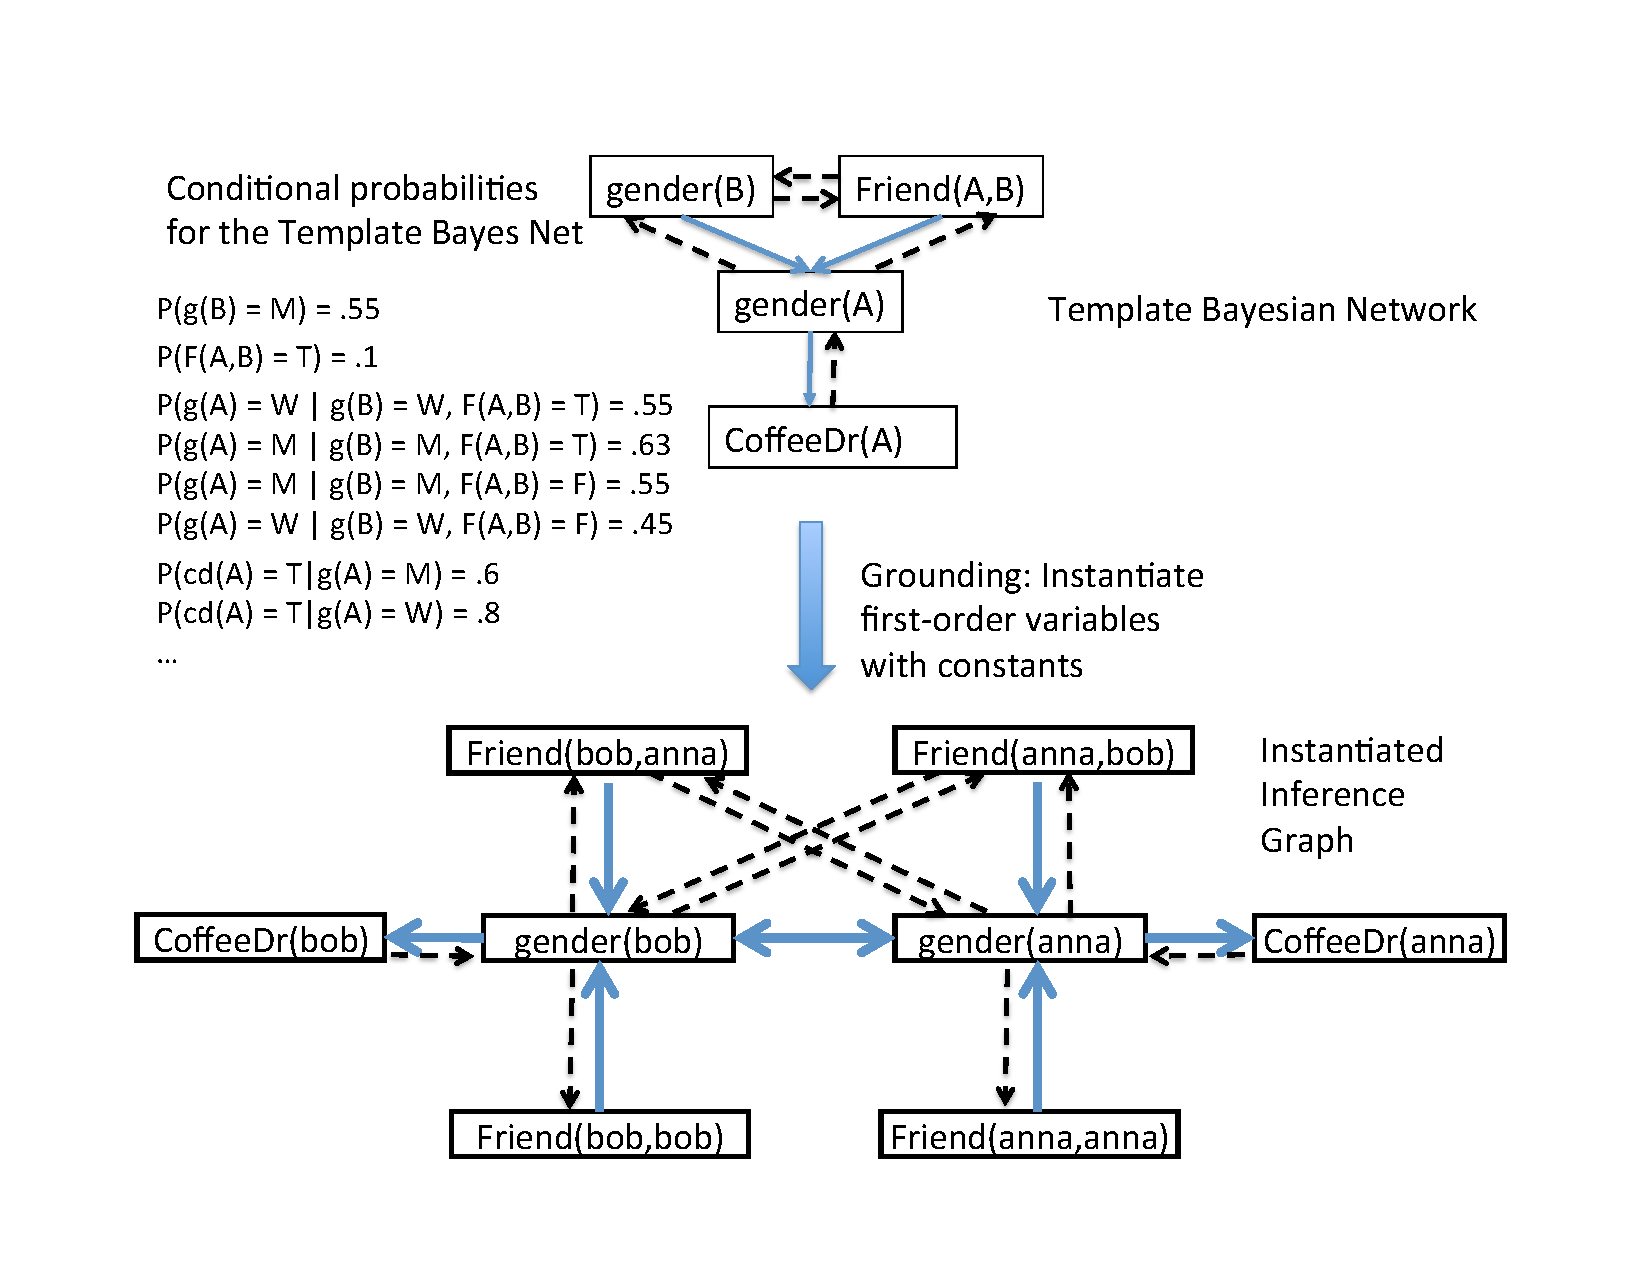
\includegraphics[width = 0.7 \textwidth]{figures/dn}
%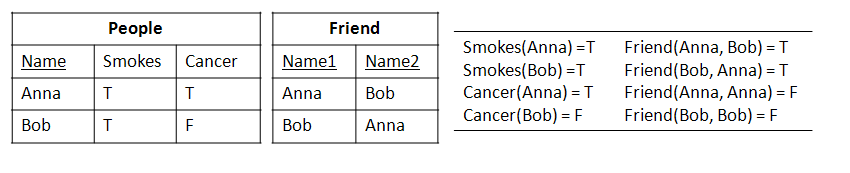
\includegraphics[width=1\textwidth]{database.png}
%}
\caption{A Bayesian/dependency template network (top) and the instantiated inference graphs (bottom). BN edges are shown as blue and solid. The BN-to-DN transformation adds the edges shown as black and dashed. Notice that grounding the BN induces a bi-directed edge between $\it{gender}(bob)$ and $\it{gender}(anna)$. \label{fig:dn}}
\end{center}
\end{figure}

 
\subsection{Relational Dependency Networks} We use  functor-based notation for graphical-relational models \cite{Poole2003}. A functor is a function or predicate symbol. Each functor has a set of values (constants) called the \textbf{domain} of the functor. In this paper we consider only functors with finite domains. A \textbf{Parametrized Random Variable} (PRV) is of the form $f(\term_{1},\ldots,\term_{k})$ where $\functor$ is a functor 
and each $\term_{i}$ is a first-order variable or a constant.
 %or a constant denoting an individual. 
 A Parametrized Bayesian Network structure is a directed acyclic graph whose nodes are PRVs. A \textbf{relational dependency network structure} (RDN) is a directed graph whose nodes are PRVs.
RDNs extend dependency networks for relational data by using knowledge-based model construction \cite{Neville2007}:
%
%\fixneeded{Oliver, my phrasing is likely wrong. My goal is to start this section with how RDNs extend DNs. How does that work?} 
%
 The first-order variables in a template RDN graph are instantiated for a specific domain of individuals to produce an {\em  instantiated} or {\em ground} propositional DN graph, the \defterm{inference graph}. Figure~\ref{fig:dn} gives a dependency network template and its grounded inference graph. An example Gibbs probability distribution for the inference graph (abbreviating functors to their first letter) is

$$P(\it{g(anna)}|\it{g(bob)}, \it{CD(anna)}, \it{F(anna,bob)},\it{F(bob,anna)},\it{F(anna,anna)}).$$


\noindent Both the structure and the parameter space of RDN models offer advantages for relational data \cite{Neville2007,Natarajan2012}: (1) Dependency network structures are well-adapted for relational data because they allow cyclic dependencies, so grounding a dependency network template is guaranteed to produce a valid dependency network.
%
%\fixneeded{Is there anything about the next paragraph that limits it to RDNs or does it all apply to DNs? If it applies to DNs, let's move it to DN section above.}
(2) Relational prediction  requires aggregating information from different linked individuals \cite{Natarajan2008}. 
%Two common approaches are combining rules \cite{Kersting2007} and aggregation functions \cite{Getoor2007c}. 
In a dependency network parameter, the aggregation encompasses the entire Markov blanket of a target node, whereas for Bayesian network parameters, the aggregation encompasses only its parents.
%
%One of the challenges for inference on relational data is that, unlike the non-relational \iid{} case, {\em a single template node may be instantiated into multiple predictors} \cite{Natarajan2008}. In the inference graph of Figure~\ref{fig:dn}, each gender of a friend of $\it{anna}$ adds one relevant predictor for the value of $\it{gender}(anna)$. The number of predictors is therefore not fixed by the model, but depends on the number of individuals related to the target individual. Relational prediction therefore requires aggregating information from different linked individuals. Two common approaches are (i) combining rules \cite{Kersting2007} and (ii) aggregation functions \cite{Getoor2007c}. In a dependency network, the aggregation encompasses the entire Markov blanket of a target node, whereas in a Bayesian network, the aggregation encompasses only its parents.
%\fixneeded{Check if we still need this after full editing.}

\section{Learning Relational Dependency Networks via Bayesian Networks}
Our algorithm for rapidly learning relational dependency networks
begins with any relational learning algorithm for Bayesian networks. We then apply a simple, fast transformation of the resulting Bayesian network to a relational dependency template. Finally we apply a closed-form computation to derive the dependency network parameters from the Bayesian structure and parameters. Figure~\ref{fig:bn-flow} shows the program flow. 
%for computing a Gibbs probability using the log-linear equation.


Converting a Bayesian network structure to a dependency network structure is simple: for each node, add an edge pointing to the node from each member of its BN Markov blanket~\cite{Heckerman2000}.  The result contains  bidirectional links between each node, its children, and its co-parents (nodes that share a child with this one). 
%
%This simply means adding edges into the node from each of its children and bidirectional links between the node and its co-parents (nodes that share a child with this one). 
This is equivalent to the standard moralization  method for converting a BN to an undirected model \cite{Domingos2009}, except that the dependency network contains bi-directed edges instead of undirected edges. Bidirected edges have the advantage that they permit  assignment of different parameters to each direction, whereas undirected edges have only one parameter.
 
Converting Bayesian network parameters to dependency network parameters is simple for propositional \iid{} data: solve for the Gibbs conditional probabilities given Bayesian network parameters. The propositional result is as follows. A \defterm{family} comprises a node and its parents. A \defterm{family configuration} specifies a value for a child node and each of its parents. For example in the Bayesian network of Figure~\ref{fig:dn}, a family configuration is 
$$\it{gender}(\A) = \Man, \it{Friend}(\A,\B) = \true, \it{gender}(\B) = \Man.$$
For propositional data, an assignment of values to the Markov blanket of a target node assigns a unique configuration for each family whose child is the target node or one of its children. Hence the Markov blanket induces a {\em unique} log-conditional probability for each such family configuration. The probability of a target node value given an assignment of values to the Markov blanket is then proportional to the exponentiated sum of these log-conditional probabilites \cite[Ch.14.5.2]{Russell2010}. 

With relational data, different family configurations such as the one above can be simultaneously instantiated, multiple times.  We adapt the propositional log-linear equation for relational data by replacing the unique log-conditional probability with the {\em expected} log-conditional probability that results from selecting an instantiation of the family configuration uniformly at random. The probability of a target node value given an assignment of values to the Markov blanket is then proportional to the exponentiated sum of the expected log-conditional probabilites. %Without this normalization, features with more instantiations carry exponentially more weight. 
We describe the resulting closed-form equation in the next section.


\begin{figure}[t]

\begin{center}
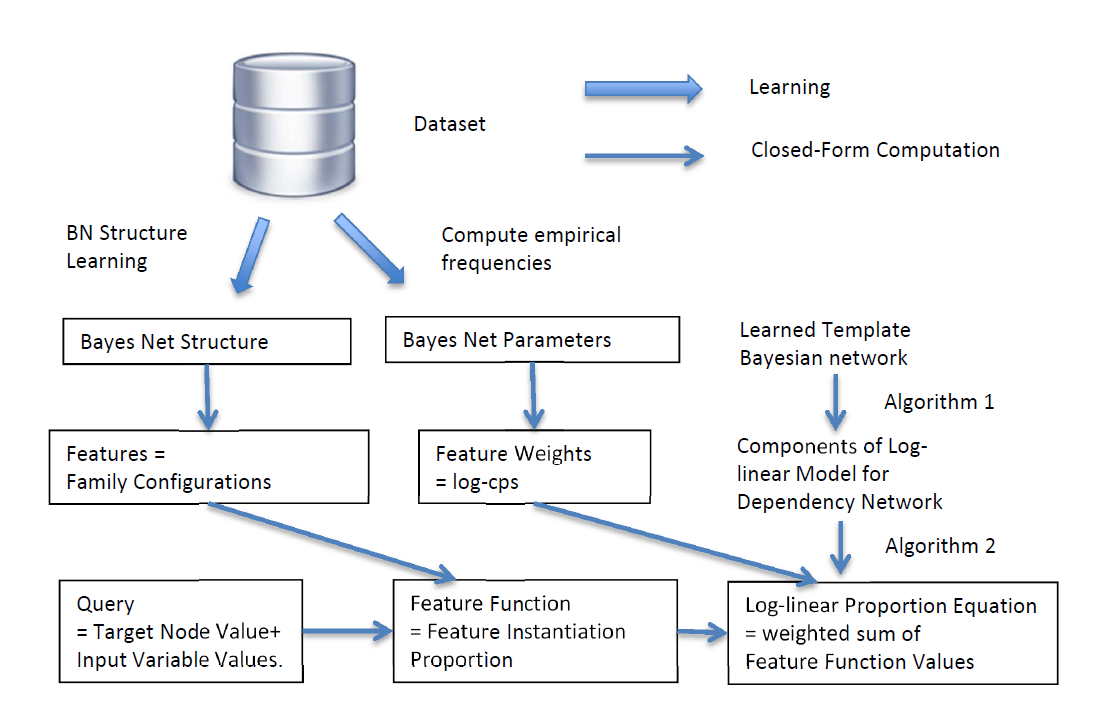
\includegraphics[width=0.7\textwidth]{bn-regress}
\caption{The program flow for computing Gibbs probabilities from a template Bayesian network. Features and weights are computed from the Bayes net. Feature function values are computed for each query. \label{fig:bn-flow}}
\end{center}

\end{figure}


\section{The Log-linear Proportion Equation} 
\label{sec:theequation}

We propose a log-linear equation, the \defterm{log-linear proportion equation}, for computing a Gibbs conditional probability for a ground target node, $\FG{\TT}$, given (i) a target value $\TV$ for the target node, (ii) a complete set of values $\QC$  for all ground terms other than the target node, and (iii) a template Bayesian network. The template structure is represented by functions that return the set of parent nodes of $\UT$, $\Pa{\UT}$, and the set of child nodes of $\UT$, $\Ch{\UT}$. The parameters of the template are
represented by the conditional probabilities of a node $\UT$ having a value $\UV$ conditional on the values of its parents, $\cprob{\UT = \UV}{\Pa{\UT} = \Prange{\UT}}$. A grounding $\grounding$ substitutes a constant for each member of a list of first-order variables. A grounding is therefore equivalent to an equality constraint $\{\A_{1} = \a_{1},\ldots, A_{k} = \a_{k}\}$. Applying a grounding to a template node defines a fully ground target node. For instance, we may have $\it{gender}(\A) \{\A = sam\} = \it{gender}(sam)$.  These are combined in the following log-linear equation:

%\noindent\fixneeded{Do we need to point out how Gibbs probabilities are sufficient building block for general probabilities?}
%
%\noindent\fixneeded{Is it informative to call it ``log-difference'' when there is no difference?}

\begin{definition}[The Log-Linear Proportion Equation]\label{def:log-diff-freq-eq}
\begin{eqnarray*}
  \Gprob{\FG{{\TT}} = \TV} {\QC} &\propto &  \\
 \sum_{\UT} \sum_{\UV,\Prange{\UT}}   
\qquad \left[ \ln \cprob{\UT = \UV}{\Pa{\UT} = \Prange{\UT}} \right] &
    \cdot &
    \Relfreq{\Appendterm{\grounding;\UT  = \UV} {\Pa{\UT} = \Prange{\UT}}} {\Qconj}
%    \Relfreq{\Appendterm{\Ground{\UI}  = \UV} {\Ground{\Pa{\UI}} = \Prange{\UT}}} {\Qconj}
\end{eqnarray*}
where 
\begin{eqnarray*}
%\UT &\mbox{varies over} &  \TT \mbox{and its children}, \\
\UT &\mathrm{varies\ over} & \Setaddterm{\{\TT\}} {\Ch{\TT}}, \\
\mbox{the singleton value} \ \UV & \mathrm{varies\ over} & \mbox{the range of}\  \UT,\\
\mbox{the vector of values} \ \Prange{\UT} & \mathrm{varies\ over} & \mbox{the product of the ranges of} \ \UT's\ \mbox{parents}, \\
\FG{\TT} = \TT \grounding&\mathrm{is} & \mbox{ is the target node grounding of template node }  \TT, \mathrm{and} \\
\Relevant{\Fvar} &\mathrm{is} & \mbox{the proportion feature function}.
\end{eqnarray*}
\end{definition}

The feature function $\Relevant{\Fvar}$ specifies the proportion of instantiations that satisfy a given family configuration, relative to all family configurations with positive links only. This proportion is computed as follows. 

\begin{enumerate}
\item For a given family configuration $(\Appendterm{\UT  = \UV} {\Pa{\UT} = \Prange{\UT}})$, let the \textbf{family  count} $$\Count{\Appendterm{\grounding;\UT  = \UV} {\Pa{\UT} = \Prange{\UT}}} {\Qconj}$$ be the number of instantiations that (a) satisfy the family configuration and the ground node values specified by $\Qconj$, and (b) are consistent with the equality constraint defined by $\grounding$. This notation is consistent with the parfactor notation of \cite{Poole2003}. 
\item The \textbf{relevant family count} $n^{r}$ is 0 if the family configuration contains a false relationship (other than the target node), else equals the feature count.
\item The \textbf{family proportion} is the relevant family count, divided by the total sum of all relevant family counts for the given family. In symbols:

\begin{equation} \notag
 \Relfreq{\Appendterm{\grounding;\UT  = \UV} {\Pa{\UT} = \Prange{\UT}}} {\Qconj} = \frac{\Relcount{\Appendterm{\grounding;\UT  = \UV} {\Pa{\UT} = \Prange{\UT}}} {\Qconj}}{\sum_{\UV',\Prange{\UT}'}\Relcount{\Appendterm{\grounding;\UT  = \UV'} {\Pa{\UT} = \Prange{\UT}'}} {\Qconj}}
\end{equation}
\end{enumerate}

It is common in statistical-relational models to restrict predictors to existing relationships only \cite{Getoor2007c,Russell2010}. The inner sum of Formula~\ref{def:log-diff-freq-eq} computes the expected log-conditional probability for a family with child node $\UT$, when we randomly select a relevant grounding of the first-order variables in the family. 
%(The random grounding must have positive links only and be consistent with the target node grounding $\grounding$.)

Definition~\ref{def:log-diff-freq-eq} has the form of a log-linear model \cite{Sutton2007}: The features of the model are the family configurations $(\Appendterm{\UT  = \UV} {\Pa{\UT} = \Prange{\UT}})$ 
%that specify the values of a child node and its parents in the template Bayesian network, 
where the child node is either the target node or one of its chldren. The feature weights are the log-conditional BN probabilities defined for the family configuration. The input variables are the values of the ground nodes other than the target nodes, specified by the conjunction $\QC$. The family count specifies how many times the feature is instantiated in the input variables (plus the target node value). The family proportion is the feature function, which maps a feature to a real value given the input variables. 
%In terms of log-linear models, this corresponds to using family configurations as features and the {\em proportion of instantiations} that satisfy a family configuration as the feature function. 
Proportions have the desirable consequence that all feature functions are normalized to the [0,1] range. 
\paragraph{Example.}
Table~\ref{table:log-diff-example} illustrates the computation of our log-linear model for predicting the gender of a new test instance ($sam$).
\begin{table}
\caption{Applying the log-linear proportion equation with the Bayesian network of Figure~\ref{fig:dn} to compute $\Gprob{\it{gender}(sam) = \Woman} {\QC}$ and $\Gprob{\it{gender}(sam) = \Man} {\QC}$. Each row represents a feature/family configuration. For the sake of the example we suppose that the conjunction $\QC$ specifies that Sam is a coffee drinker, has 60 male friends, and 40 female friends. $CP$ refers to the conditional probability BN parameter of Figure~\ref{fig:dn}. For the feature weights $w \equiv \ln(CP)$.
\label{table:log-diff-example}}
\centering
%\resizebox{1.1\textwidth}{!}{
\begin{tabular}{l@{\hspace{.1in}}l@{\hspace{.1in}}r@{\hspace{.1in}}r@{\hspace{.1in}}r@{\hspace{.1in}}r}
%%%%%% DO NOT MODIFY THIS FILE DIRECTLY %%%%%%
%%%%%% IT IS GENERATED BY apply-eqs.py %%%%%%
\\\hline
{\setlength{\tabcolsep}{0pt}\begin{tabular}{l}Child \\Value \end{tabular}}&{\setlength{\tabcolsep}{0pt}\begin{tabular}{l} Prior \\ Prob. \end{tabular}}&Parent State&{\setlength{\tabcolsep}{0pt}\begin{tabular}{l} Cond. \\ Prob.\end{tabular}}&$w\;\;$&$\Relevant{\Fvar}$&$w \times \Relevant{\Fvar}$&$\Relevant{\Cvar}$&$w \times \Relevant{\Cvar}$ \\\hline
$cd(sam) = \true$&$0.70\;$&{\setlength{\tabcolsep}{0pt}\begin{tabular}{l}$ g(sam) = \Woman$\end{tabular}}&$0.80\;\,$&$0.13$&$1.0$&$0.13\;\;$&$1$&$0.13\;\;$ \\
$cd(sam) = \false$&$0.30\;$&{\setlength{\tabcolsep}{0pt}\begin{tabular}{l}$g(sam) = \Woman$ \end{tabular}}&$0.20\;\,$&$-0.40$&$0.0$&$0.00\;\;$&$0$&$0.00\;\;$ \\
$g(sam) = \Woman$&$0.45\;$&{\setlength{\tabcolsep}{0pt}\begin{tabular}{l}$ g(B) = \Woman,$\\ $F(sam,B) = \true$\end{tabular}}&$0.55\;\,$&$0.20$&$0.4$&$0.08\;\;$&$40$&$8.02\;\;$ \\
$g(sam) = \Woman$&$0.45\;$&{\setlength{\tabcolsep}{0pt}\begin{tabular}{l}$ g(B) = \Man,$\\ $ F(sam,B) = \true$\end{tabular}}&$0.37\;\,$&$-0.19$&$0.6$&$-0.11\;\;$&$60$&$-11.74\;\;$ \\
$g(sam) = \Woman$&$0.45\;$&{\setlength{\tabcolsep}{0pt}\begin{tabular}{l} n/a\end{tabular}}&$\mathrm{n/a}\;\,$&$-0.79$&$1.0$&$-0.79\;\;$&$1$&$-0.79\;\;$ \\\hline
\multicolumn{6}{l}{Sum ($\ln \Gprob{\it{gender}(sam) = \Woman} {\QC}$)}&$-0.70\;\;$&&$-4.38\;\;$ \\\hline
$cd(sam) = \true$&$0.70\;$&{\setlength{\tabcolsep}{0pt}\begin{tabular}{l}$ g(sam) = \Man$\end{tabular}}&$0.60\;\,$&$-0.15$&$1.0$&$-0.15\;\;$&$1$&$-0.15\;\;$ \\
$cd(sam) = \false$&$0.30\;$&{\setlength{\tabcolsep}{0pt}\begin{tabular}{l}$ g(sam) = \Man$\end{tabular}}&$0.40\;\,$&$0.28$&$0.0$&$0.00\;\;$&$0$&$0.00\;\;$ \\
$g(sam) = \Man$&$0.55\;$&{\setlength{\tabcolsep}{0pt}\begin{tabular}{l}$ g(B) = \Woman,$\\ $F(sam,B) = \true$\end{tabular}}&$0.45\;\,$&$-0.20$&$0.4$&$-0.08\;\;$&$40$&$-8.02\;\;$ \\
$g(sam) = \Man$&$0.55\;$&{\setlength{\tabcolsep}{0pt}\begin{tabular}{l}$ g(B) = \Man,$\\ $ F(sam,B) = \true$\end{tabular}}&$0.63\;\,$&$0.13$&$0.6$&$0.08\;\;$&$60$&$8.14\;\;$ \\
$g(sam) = \Man$&$0.55\;$&{\setlength{\tabcolsep}{0pt}\begin{tabular}{l} n/a \end{tabular}}&$\mathrm{n/a}\;\,$&$-0.59$&$1.0$&$-0.59\;\;$&$1$&$-0.59\;\;$ \\\hline
\multicolumn{6}{l}{Sum ($\ln \Gprob{\it{gender}(sam) = \Man} {\QC}$)}&$-0.75\;\;$&&$-0.63\;\;$ \\\hline

\end{tabular}
%}
\end{table}



\paragraph{Estimating Bayes net parameters.}
The Bayesian network parameters can be estimated by applying the maximum likelihood principle, which entails using the empirical conditional frequencies observed in an input relational database \cite{Schulte2011,Schulte2014}. 
 Although there is theoretical justification for using the empirical frequencies, the ultimate test is whether the method can achieve comparable accuracy and greater speed than prior methods of computing relational dependency networks. In the next section, we empirically compare these methods.
 
 
%The Bayes net parameters can be estimated using the empirical conditional frequencies observed in an input dataset $\FG{\Delta}$: The parameter estimate for a family configuration is the number of instantiations of that family configuration in $\FG{\Delta}$, divided by the sum of all instantiation counts for that family that agree on the parent values and vary the child values. In our notation, the estimate is defined by
%
%\newcommand{\CTPa}{\Count{\Appendterm{\TT = \TV} {\Pa{\TT} = \Prange{\TT}}}  {\FG{\Delta}}}
%\newcommand{\CTPb}{\Count{\Appendterm{\TT = \TV'} {\Pa{\TT} = \Prange{\TT}}}  {\FG{\Delta}}}
%
%\begin{equation} \label{eq:frequencies}
%\estcprob{\TT = \TV} {\Pa{\TT} = \Prange{\TT}} {\FG{\Delta}} = 
%    \frac{\CTPa}
%           {\sum_{\TV' \in \Range{\TT}}\CTPb}.
%\end{equation}
%
%A theoretical justification for using the observed conditional frequencies is that these estimates maximize a pseudo-likelihood function that measures how well a template BN matches an input dataset \cite{Schulte2011,Schulte2013}. The pseudo-likelihood can be interpreted as the expected value of the log-likelihood of a random grounding of the BN nodes in the template model.
%
%Although this theoretical justification assures us of the conceptual coherence of Equation~\ref{def:log-diff-freq-eq}, the ultimate test is whether the method can achieve comparable accuracy and greater speed than prior methods of computing relational dependency networks. In the next section, we empirically compare these methods.

\section{Empirical Comparison with Functional Gradient Boosting}\label{sec:empirical-comparison}

The next section describes experiments that compare learning RDNs via Bayesian networks with functional gradient methods for learning relational dependency networks. Boosting methods follow the traditional approach to learning dependency networks, which is to learn a collection of separate discriminative models, one for each node in the network \cite{Heckerman2000}. Functional gradient boosting has been shown to perform well on small datasets previously \cite{Khot2011,Natarajan2012}; our experiments provide new new tests of this method on medium to large datasets. 

\subsection{Experimental Conditions and Metrics}\label{sec:conditions}

All experiments were done on with 8GB of RAM and a single Intel Core 2 QUAD Processor Q6700 with a clock speed of 2.66GHz (there is no hyper-threading on this chip). The operating system was Linux Centos 2.6.32. Code was written in Java, JRE 1.7.0. All code and datasets are available~\cite{bib:jbnsite}. 

\subsubsection{Datasets}
We used 
5 benchmark real-world databases. For more details please see the references in \cite{Schulte2012}. Summary statistics appear in Table~\ref{table:learning-times}.

\begin{description}

\item[MovieLens Databases] MovieLens is a  commonly-used rating dataset (www.grouplens.org). %We added more related attribute information about the actors, directors and movies from the Internet Movie Database (IMDB) (www.imdb.com, July 2013).
It contains two entity sets, Users and Movies. For each user and movie that appears in the database, all available ratings are included. MovieLens(1M) contains 1M ratings, 3,883 Movies, and 6,039 Users. MovieLens(0.1M) contains about 0.1M ratings, 1,682 Movies, and 941 Users. We did not use the binary genre predicates because they are easily learned with exclusion rules.


\item[Mutagenesis Database] This dataset is widely used in Inductive Logic Programming research. 
It contains information on Atoms, Molecules, and Bonds between them. We use the discretization of \cite{Schulte2012}.

\item[Hepatitis Database] This data is a modified version of the PKDD02 Discovery Challenge database. %, which includes removing tests with null values. 
The database contains information on the laboratory examinations of hepatitis B and C infected patients. 

\item[Mondial Database] 
This dataset contains data from multiple geographical web data sources. 


\item[UW-CSE Database] This dataset lists facts about the Department of Computer Science and Engineering at the University of Washington, such as entities (e.g., $Person$, $Course$) and the relationships (i.e. $AdvisedBy$, $TaughtBy$).

\end{description}

\subsubsection{Methods Compared} Functional gradient boosting is a state-of-the-art method for applying discriminative learning to build a generative graphical model. The local discriminative models are  ensembles of relational regression trees \cite{Khot2011}. Our experiments used the Boostr implementation of relational gradient boosting \cite{Khot2013}. The current implementation does not support multi-class boosting, so following previous experiments \cite{Khot2011}, we limited our comparison to {\em binary predicates}, i.e., functors that can take on only two possible values (e.g., $\it{AdvisedBy}$). We compared the following three learning methods.

\begin{description}
\item[RDN\_Bayes] Learns a Bayesian network, then converts it to a relational dependency network as described above.
\item[RDN\_Boost] The state-of-the-art gradient boosting method designed for learning RDNs. Information from ground nodes that are linked to the target node is aggregated with functions $count, max, average$ and existential quantification \cite{Natarajan2012}.
\item[MLN\_Boost] The state-of-the-art gradient boosting method designed for learning Markov Logic Networks. It takes as input a  list of target predicates for analysis. To construct an RDN, we provide each binary predicate as a single target predicate in turn. Information from ground nodes that are linked to the target node is aggregated with a log-linear model derived from Markov Logic Networks.
\end{description}
%Used as an RDN learner in this way, the main difference of MLN\_Boost with RDN\_Boost is that it aggregates information from ground nodes that are linked to the target node using a log-linear model derived from Markov Logic Networks. 
We followed the Boostr instructions for creating the background .bk file and used the default settings. We experimented with alternative settings but they did not improve the performance of the boosting methods.


To obtain the BN structure for RDN\_Bayes, the learn-and-join algorithm~\cite{Schulte2012} was applied to each benchmark database. The BN parameters were computed from the empirical conditional frequencies in the database using previously-published algorithms~\cite{Schulte2014}. 
%The resulting structure and parameters were used for all methods in this experiment. 

\subsubsection{Prediction Metrics}
We follow \cite{Khot2011} and evaluate the algorithms using conditional log likelihood (CLL) and AUC-PR (Area Under Precision-Recall Curve). AUC-PR is appropriate when the target predicates features a skewed distribution as is typically the case with relationship predicates. %These metrics have been used in previous evaluations of MLN learning~\cite{Domingos2007,Schulte2012}.  
For each fact $\FG{\TT} = \TV$ in the test dataset, we evaluate the accuracy of the predicted Gibbs probability $\Gprob{\FG{\TT} = \TV} {\QC}$, where $\QC$ is a complete conjunction for all ground terms other than $\FG{\TT}$. Thus $\QC$ represents the values of the input variables as specified by the test dataset.
%For classification accuracy, a model's prediction is scored as correct if the true value of the ground term in the test dataset receives the highest Gibbs probability. 
CLL is the average of the logarithm of the Gibbs probability for each ground truth fact in the test dataset. For the gradient boosting method, we used the AUC-PR and likelihood scoring routines included in Boostr.
%Thus $\exp(CLL)$ is the geometric mean of the Gibbs probabilities.\footnote{The geometric mean of a list of numbers $x_{1},\ldots,x_{n}$ is $(\prod_{i} x_{i})^{1/n}$.} 


Both metrics are reported as averages over all binary predicates. The learning methods were evaluated using 5-fold cross-validation. Each database was split into 5 folds by randomly selecting entities from each entity table, and restricting the relationship tuples in each fold to those involving only the selected entities  (i.e., subgraph sampling~\cite{Schulte2012}). The models were trained on 4 of the 5 folds, then tested on the remaining one. All results are averages from 5-fold cross validation, over all descriptive attributes in the database. 


\subsection{Results} 

Table~\ref{table:learning-times} shows learning times for the different methods. For the boosting method, we added together the learning times for each target predicate. The total learning times are not directly comparable because Bayes net learning simultaneously learns a joint model for all predicates. We therefore report total learning time divided by the number of all predicates for RDN\_Bayes, and total learning time divided by the number of binary predicates for the boosting methods. The numbers of predicates are given in the second column.
 % Table generated by Excel2LaTeX from sheet 'learning time table May 12'
\begin{table}[htbp]
  \centering
  \caption{Learning Time (Sec) Per Predicate}
    \begin{tabular}{|l|p{2cm}|r|r|r|r|}
\hline
     Dataset & all predicates / binary predicates & \# tuples & RDN\_Bayes & RDN\_Boost & MLN\_Boost \\ \hline
    UW    & 14/4  & 612   & 0.74$\pm$0.05 & 14.57$\pm$0.39 & 19.27$\pm$0.77  \\
    Mondial & 18/4  & 870   & 101.53$\pm$6.90 & 27.21$\pm$0.98 & 41.97$\pm$1.03 \\
    Hepatitis & 19/7  & 11,316 & 285.71$\pm$20.94 & 250.61$\pm$5.32 & 229.73$\pm$2.04  \\
    Mutagenesis & 11/6  & 24,326 & 0.70$\pm$0.02 & 117.70$\pm$6.37 & 48.65$\pm$1.34 \\ 
    MovieLens(0.1M) & 7/2   & 83,402 & 1.11$\pm$0.08 & 2638.71$\pm$272.78 &  1866.605$\pm$112.54\\
    MovieLens(1M) & 7/2   & 1,010,051 & 1.12$\pm$0.10 & $>$24 hours & $>$24 hours \\ \hline
  
    \end{tabular}%
  \label{table:learning-times}%
\end{table}%
%
%
%\begin{table}[htbp]
%  \centering
%  \caption{Learning Time (Sec) Per Predicate}
%    \begin{tabular}{|l|p{2cm}|r|r|r|r|}
%\hline
%     Dataset & all predicates / binary predicates & \# tuples & RDN\_Bayes & RDN\_Boost & MLN\_Boost \\ \hline
%    UW    & 14/4  & 612   & 0.74$\pm$0.05 & 14.57$\pm$0.39 & 19.27$\pm$0.77  \\
%    Mondial & 18/4  & 870   & 101.53$\pm$6.90 & 27.21$\pm$0.98 & 41.97$\pm$1.03 \\
%    Hepatitis & 19/7  & 11,316 & 285.71$\pm$20.94 & 250.61$\pm$5.32 & 229.73$\pm$2.04  \\
%    Mutagenesis & 11/6  & 24,326 & 0.70$\pm$0.02 & 117.70$\pm$6.37 & 48.65$\pm$1.34 \\ 
%    MovieLens(0.1M) & 7/2   & 83,402 & 1.11$\pm$0.08 & 2638.71$\pm$272.78 &  1866.605$\pm$112.54\\
%    MovieLens(1M) & 7/2   & 1,010,051 & 1.12$\pm$0.10 & $>$24 hours & $>$24 hours \\ \hline
%  
%    \end{tabular}%
%  \label{table:learning-times}%
%\end{table}%


Table~\ref{table:learning-times} shows that RDN\_Bayes scales very well with the number of data tuples: even the large MovieLens dataset with 1M records can be analyzed in seconds. Learning separate discriminative models  scales well with the number of predicates, which is consistent with findings from  propositional learning \cite{Heckerman2000}. Bayes net learning slows down more as more predicates are included, since it learns a joint model over all predicates simultaneously. However, the learning time remains feasible (see also \cite{Schulte2012}). Bayesian network learning scales well in the number of data points because it provides closed-form parameter estimation and hence closed-form model scoring. Unlike propositional iid data, relational data are represented in multiple tables, so model evaluation requires expensive combining of information from different tables \cite{Neville2007}. Compared to learning separate discrimative models, Bayesian network explores a more complex model space, but  model evaluation is much faster. 
% Table generated by Excel2LaTeX from sheet 'temp'
\begin{table}[htbp]
 \centering
  \caption{Average Conditional Log-Likelihood}
    \begin{tabular}{|r|r|r|r|r|r|} \hline
    \textbf{CLL} & UW    & Mondial  & Hepatitis & Mutagenesis  & MovieLens(0.1M) \\ \hline
   RDN\_Boost & -0.29$\pm$0.02 & -0.48$\pm$0.03 & -0.51$\pm$0.00 & -0.43$\pm$0.02 & -0.58$\pm$0.05 \\
    MLN\_Boost & -0.16$\pm$0.01 & -0.40$\pm$0.05 & -0.52$\pm$0.00 & -0.24$\pm$0.02 & -0.38$\pm$0.06 \\
    RDN\_Bayes & \textbf{-0.01$\pm$0.00} & \textbf{-0.25$\pm$0.06} & \textbf{-0.39$\pm$0.10} & \textbf{-0.22$\pm$0.07} & \textbf{-0.30$\pm$0.02} \\ \hline
    \end{tabular}%
  \label{table:cll}%
%\end{table}%

% Table generated by Excel2LaTeX from sheet 'temp'
%\begin{table}[htbp]
 \centering 
 \vspace{0.1cm}
 \caption{Average Area Under Precision-Recall Curve}
    \begin{tabular}{|r|r|r|r|r|r|} \hline
    \textbf{AUC-PR} & UW    & Mondial  & Hepatitis & Mutagenesis  & MovieLens(0.1M) \\ \hline
    RDN\_Boost & 0.32$\pm$0.01 & 0.27$\pm$0.01 & \textbf{0.71$\pm$0.02} & 0.63$\pm$0.02 & 0.52$\pm$0.03 \\
    MLN\_Boost & 0.52$\pm$0.01 & 0.44$\pm$0.05 & \textbf{0.71$\pm$0.02} & \textbf{0.83$\pm$0.05} & 0.52$\pm$0.05 \\
    RDN\_Bayes & \textbf{0.89$\pm$0.00} & \textbf{0.79$\pm$0.07} & 0.55$\pm$0.11 & 0.50$\pm$0.10 & \textbf{0.65$\pm$0.02} \\ \hline
    \end{tabular}%
  \label{table:AUC}%
\end{table}%

Tables~\ref{table:cll} and~\ref{table:AUC} show results for predictive accuracy. Our system resources did not suffice for evaluating the metrics on MovieLens(1M).  In terms of the likelihood assigned to the ground truth predicate value, the Bayes net method outperforms both boosting methods on all datasets (Table~\ref{table:cll}). In terms of the precision-recall curve, the Bayes net method performs substantially better than both on three datasets, and substantially worse on the two others (Table~\ref{table:AUC}). This is a satisfactory performance because boosting is a powerful method for achieving accurate predictions, and was applied to each target predicate individually to produce a tailored discriminative model. Bayesian network learning simultaneously constructed a joint model for all predicates, and used simple maximum likelihood estimation for parameter values.
 Our overall conclusion is that \emph{Bayes net learning scales much better to large datasets, and provides competitive accuracy in predictions.} 

In addition to scalability, Bayesian networks offer two more advantages. First, learning easily extends to attributes with more than two possible values. Second, the parameters and the predictions derived from them are easily interpretable. The ensemble of regression trees is more difficult to interpret, as the inventors of the boosting method noted  \cite{Natarajan2012}.
%; as the inventors of the boosting method put it, ``we sacrifice comprehensibility for better predictive performance'' \cite{Natarajan2012}. 

\section{Related Work}


Dependency networks were introduced in \cite{Heckerman2000} and relational dependency networks in \cite{Neville2007}. 
Heckerman {\em et al.} compare Bayesian, Markov and dependency networks for nonrelational data. 

\emph{Bayesian networks.} There are several proposals for defining directed relational template models, based on graphs with directed edges or rules in clausal format \cite{Kersting2007,Getoor2007c}. Defining the probability of a child node conditional on multiple instantiations of a parent set requires the addition of combining rules \cite{Kersting2007} or aggregation functions \cite{Getoor2007c}. 
%As described by \cite{Kersting2007}, aggregate functions can be added to a Parametrized Bayesian network by including functor nodes with aggregates. 
Combining rules such as the arithmetic mean~\cite{Natarajan2008} combine global parameters with a local scaling factor, as does our log-linear model. In terms of combining rules,  our model uses the {\em geometric mean} rather than the arithmetic mean.\footnote{The geometric mean of a list of numbers $x_{1},\ldots,x_{n}$ is $(\prod_{i} x_{i})^{1/n}$. The logarithm of the geometric mean is therefore $1/n \sum_{i} \ln x_{i}$. Thus geometric mean = exp(average (logs)).} To our knowledge, the geometric mean has not been used before as a combining rule for relational data.  
%Another difference with template Bayesian networks is that the geometric mean is applied to the entire Markov blanket of the target node, whereas usually a combining rule applies only to the parents of the target node. 

\emph{Markov Networks.} Markov Logic Networks (MLNs) provide a logical template language for undirected graphical models. 
Richardson and Domingos propose transforming a Bayesian network to a Markov Logic network using moralization, with log-conditional probabilities as weights \cite{Domingos2009}. 
This is also the standard BN-to-MLN transformation recommended by the Alchemy system \cite{bib:bayes-convert}. A discriminative model can be derived from any MLN \cite{Domingos2009}.  The structure transformation was used in previous work \cite{Schulte2012}, where MLN parameters were learned, not computed in closed-form from BN parameters. The Gibbs conditional probabilities derived from an MLN obtained from converting a Bayesian network are the same as those defined by our log-linear Formula~\ref{def:log-diff-freq-eq}, {\em if} counts replace proportions as feature functions \cite{Schulte2011}. There is no MLN whose discriminative model is equivalent to our log-linear equation with  proportions as feature functions.\footnote{Disclaimer: A preliminary version of this paper was presented at the StarAI 2012 workshop, with no archival proceedings. We are indebted to workshop reviewers and participants for helpful comments.}
 


\section{Conclusion and Future Work} 
\label{sec:conclusion}
Relational dependency networks offer important advantages for modelling relational data. We proposed a novel approach to learning dependency networks: first learn a Bayesian network, then perform a closed-form transformation of the Bayesian network to a dependency network. The key question is how to transform BN parameters to DN parameters. We introduced a new relational adapation of the standard BN log-linear equation for the probability of a target node conditional on an assigment of values to its Markov blanket. The new log-linear equation uses a sum of expected values of BN log-conditional probabilities, with respect to a random instantiation of first-order variables. This is equivalent to using feature instantiation proportions as feature functions. We compared our approach to state-of-the-art functional gradient boosting methods  on five benchmark datasets. Learning RDNs via BNs scales much better to large datasets than with boosting, and provides competitive accuracy in predictions.

Learning a collection of discriminative models and learning a Bayesian network learning are two very different approaches to constructing dependency networks, each with strengths and weaknesses. There are various options for hybrid approaches that combine the strengths of both. (1) Fast Bayesian network learning methods can be used to select features. Discriminative learning methods should work  faster restricted to the BN Markov blanket of a target node. (2) The Bayesian network can provide an initial dependency network structure. Gradient boosting can then be used to fine-tune a discriminative model of a child node given parent nodes, replacing a flat conditional probability table. In sum, learning relational dependency networks via Bayesian networks is a novel approach that offers promising advantages for  interpretability and scalability.

%\section*{Acknowledgements} 
%%This work was supported by Discovery Grants to Oliver Schulte from the Natural Science and Engineering Council of Canada. Zhensong Qian was supported by a grant from the China Scholarship Council. 
%A preliminary version of this paper was presented at the StarAI 2012 workshop. We are indebted to workshop reviewers and participants for helpful comments.

\bibliographystyle{plain}
\bibliography{master}
\end{document}
